\documentclass[11pt,a4paper]{article}

\usepackage[margin=0.92in]{geometry}
\usepackage{amsmath,amssymb,amsthm,mathtools}
\usepackage{booktabs}
\usepackage{array}
\usepackage{graphicx}
\usepackage{xcolor}
\usepackage{enumitem}
\usepackage{microtype}
\usepackage[hidelinks,
  pdftitle={Morgenstern Gate-Bit Conservation, Complex-FFT vs. Bounded-Exponent Finite-Field NTT Precision Dichotomy, and Exact Straight-Line Circuit Certificates from the N(log N)^(1/2) Fourier Exponent},
  pdfauthor={Lluis Eriksson}
]{hyperref}

\newtheorem{theorem}{Theorem}[section]
\newtheorem{proposition}[theorem]{Proposition}
\newtheorem{lemma}[theorem]{Lemma}
\newtheorem{corollary}[theorem]{Corollary}
\theoremstyle{definition}
\newtheorem{definition}[theorem]{Definition}
\theoremstyle{remark}
\newtheorem{remark}[theorem]{Remark}

\newcommand{\QQ}{\mathbb{Q}}
\newcommand{\RR}{\mathbb{R}}
\newcommand{\CC}{\mathbb{C}}
\newcommand{\ZZ}{\mathbb{Z}}
\newcommand{\NN}{\mathbb{N}}
\newcommand{\FF}{\mathbb{F}}
\newcommand{\diag}{\operatorname{diag}}
\newcommand{\certschema}{\texttt{FOURIER-GATE-CERT-1.0}}
\emergencystretch=1.5em

\title{\bfseries Morgenstern Gate--Bit Conservation, Complex-FFT vs.\ Bounded-Exponent Finite-Field NTT Precision Dichotomy, and Exact Straight-Line Circuit Certificates from the $N(\log N)^{1/2}$ Fourier Exponent}

\author{Lluis Eriksson\thanks{Independent researcher (Sweden). Manuscript and figures: CC-BY-4.0; code, Lean~4 proofs, and certificates: MIT license. Prepared with transparent AI assistance via Google Antigravity; all proofs, verifiers, and tests were independently compiled and verified locally. Repository: \url{https://github.com/lluiseriksson/fourier-sqrtlog-certificates}.}}

\date{November 25, 2026}

\begin{document}
\maketitle

\begin{abstract}
On November 24, 2026, OpenAI (\texttt{openai/math}) proved that the minimum number of binary linear gates for the discrete Fourier transform (DFT) of any finite abelian group of order $N$---as well as $J$ independent batched transforms and formal polynomial multiplication---is $N(\log_2 N)^{1/2+o(1)}$ over fields with unrestricted scalar constants, surpassing Cooley--Tukey's $O(N\log_2 N)$ barrier by a factor of $\sqrt{\log_2 N}$. Here we prove four exact quantitative, architectural, and certification consequences of this result, backed by an $18$-theorem zero-dependency Lean~4 algebraic lemma ledger (\texttt{v4.35.0}, $0$~\texttt{sorry}, $0$~\texttt{Classical.choice}, $0$~warnings) and a pure-stdlib zero-float straight-line DAG verifier (\certschema{}). First, combining character orthogonality $|\det(F_G^{\oplus J})| = N^{JN/2}$ with Morgenstern's $1973$ volume bound yields the exact \emph{Gate--Bit Conservation Law} $L \cdot \log_2 C \ge \frac{1}{2} J N \log_2 N$ for every complex linear circuit with gate-weight bound $|a|+|b| \le C$. Consequently, any circuit achieving OpenAI's $L \le c_0 J N (\log_2 N)^{1/2+\varepsilon}$ bound over $\CC$ must suffer super-polynomial scalar weight blow-up $C(N) \ge 2^{\frac{1}{2c_0}(\log_2 N)^{1/2-\varepsilon}}$, restoring an $\Omega(J N \log_2 N)$ gate-times-dynamic-range product in fixed-point or exact-integer complex arithmetic. By contrast, over a fixed prime field $\FF_q$ (e.g.\ ML-KEM/Kyber $q=3329$ at $w=12$~bits or ML-DSA/Dilithium $q=8380417$ at $w=23$~bits), any bounded-exponent abelian product group $G$ of order $N = 2^k$ with $\exp(G) \mid (q-1)$ (such as $(\ZZ/256\ZZ)^m$ over $\FF_{3329}$) escapes the Archimedean determinant constraint at constant modulus width $w$ independent of $N$ (whereas cyclic NTTs $G = \ZZ/N\ZZ$ force $q > N$ and $w \ge k$). Second, for OpenAI's rectangular rank--support separation $\Delta_{\mathrm{rect}}(L) = \sqrt{1+L^2}-1$, we prove the unconditional rational bracket $\frac{L^2}{2+L} < \Delta_{\mathrm{rect}}(L) < \frac{L^2}{2}$ for all $L > 0$ and exact evaluation $\Delta_{\mathrm{rect}}\bigl(\frac{2uv}{u^2-v^2}\bigr) = \frac{2v^2}{u^2-v^2}$. Third, we establish exact finite-$N$ crossovers ($k^* = c_0^2$) and bilinear vs.\ fixed-kernel circulant/Toeplitz budgets. Fourth, we prove soundness and completeness of \certschema{}, which independently executes and certifies $16$ exact certificates across four modes---including classical $N\log_2 N$ acyclic DAGs for Walsh--Hadamard $H_4, H_8, H_{16}$ over $\QQ$ and prime-field NTTs over $\FF_{17}$, $\FF_{257}$, and ML-KEM/Kyber $\FF_{3329}$ ($N=8,16$) with exact circulant convolution checks---in $\le 5.58\,\mathrm{ms}$ while rejecting $50/50$ live adversarial red-team attacks.
\end{abstract}

\section{Introduction}

Since Cooley and Tukey~\cite{cooley1965algorithm} established $O(N\log_2 N)$ linear-gate circuits for the discrete Fourier transform (DFT), whether the logarithmic factor $\log_2 N$ was optimal for unrestricted linear circuits remained a central open question of algebraic complexity. In $1973$, Morgenstern~\cite{morgenstern1973note} proved that if every binary linear gate $u \mapsto a u_1 + b u_2$ has bounded complex weight $|a| + |b| \le C$, then any circuit computing the $N\times N$ DFT matrix $F_N$ over $\CC$ requires at least $\frac{1}{2\log_2 C} N \log_2 N$ gates.

On November 24, 2026, OpenAI~\cite{openai2026dft} resolved the unrestricted model over every field $K$ containing the required roots of unity (with $N$ invertible in $K$): for any $J \ge 1$ finite abelian groups $G_1,\dots,G_J$ of common order $N \ge 2$, the minimum binary linear gate count $C_K(T)$ of their direct-sum Fourier transform $T = \bigoplus_{j=1}^J F_{G_j}$ satisfies
\begin{equation}\label{eq:oai-dft}
  c\, J N \sqrt{\log_2 N} \;\le\; C_K(T) \;\le\; C_\varepsilon\, J N (1 + \log_2 N)^{1/2+\varepsilon}
\end{equation}
for every $\varepsilon > 0$ (and the same logarithmic exponent $1/2$ governs formal polynomial multiplication). The lower bound relies on OpenAI's companion Euclidean tensor geometry~\cite{openai2026euclidean}, testing rank and support jointly on a width-$1$, height-$L$ rectangle where a character table costs $(L + \sqrt{1+L^2})\log_2 N$ versus $(L+1)\log_2 N$ for a permutation matrix.

This breaking of the $N\log_2 N$ gate barrier raises three concrete quantitative and certification questions:
\begin{enumerate}[leftmargin=1.8em,itemsep=2pt]
  \item \textbf{Reconciling~\eqref{eq:oai-dft} with Morgenstern's $N\log_2 N$ barrier:} How fast must scalar gate weights grow in any $O(JN(\log_2 N)^{1/2+\varepsilon})$ circuit over $\CC$, and for which finite abelian groups $G$ do fixed-modulus prime-field Number-Theoretic Transforms (NTTs) over post-quantum moduli such as ML-KEM/Kyber~\cite{nist2024mlkem} and ML-DSA/Dilithium~\cite{nist2024mldsa} avoid this blow-up?
  \item \textbf{Exact rational geometry of the rectangular rank--support test:} Can the irrational separation $(\sqrt{1+L^2}-1)\log_2 N$ driving~\eqref{eq:oai-dft} be tightly bracketed and evaluated purely over $\QQ$ without square roots?
  \item \textbf{Zero-float straight-line DAG certification:} How can explicit binary linear circuits over $\QQ$ and prime fields $\FF_q$ (together with circulant/Toeplitz convolution checks) be independently executed and verified from scratch with zero floating-point arithmetic?
\end{enumerate}

\paragraph{Explicit Scope Separation.}
Our analytical theorems (Theorems~\ref{thm:conservation}--\ref{thm:verifier}) are proved completely in Section~\ref{sec:results}. The companion Lean~4 module (\texttt{lean/FourierSqrtLog.lean}, Section~\ref{sec:lean}) formally machine-checks the $18$ cleared-denominator integer, divisibility, and crossover algebraic lemmas underlying those proofs; it does \emph{not} formalize linear circuits, complex determinants, Morgenstern's volume theorem, or the Python verifier inside Lean~4. Concrete straight-line DAG evaluation over $\QQ$ and $\FF_q$ is carried out by the audited pure-stdlib verifier \certschema{} (Section~\ref{sec:experiments}).

\section{Main Exact-\texorpdfstring{$\QQ$}{Q} and Exact-\texorpdfstring{$\FF_q$}{Fq} Theorems}\label{sec:results}

\subsection{Morgenstern Gate--Bit Conservation and the Complex-FFT vs.\ Bounded-Exponent NTT Dichotomy}

\begin{theorem}[Gate--Bit Conservation Law and Bounded-Exponent Precision Dichotomy]\label{thm:conservation}
Let $G_1,\dots,G_J$ be finite abelian groups of common order $N = 2^k \ge 2$ ($J \ge 1, k \ge 1$), and let $T = \bigoplus_{j=1}^J F_{G_j}$ be their batched unnormalized Fourier transform over $\CC$ (so $F_{G_j} F_{G_j}^\dagger = N I_N$ for every $j$).
\begin{enumerate}[leftmargin=1.8em,itemsep=2pt]
  \item \textbf{Universal Gate--Bit Conservation Law:} In any acyclic binary linear circuit over $\CC$ computing $T$ with $L$ gates of the form $z = \alpha u + \beta v$ satisfying $|\alpha| + |\beta| \le C$ ($C = 2^b > 1$, so $b = \log_2 C > 0$ bits of scalar dynamic range per gate) and unscaled wire readouts (or with any output scaling counted among the $L$ bounded-weight gates),
  \begin{equation}\label{eq:conservation}
    L \cdot b = L \cdot \log_2 C \;\ge\; \frac{1}{2}\, J N \log_2 N = \frac{1}{2}\, J N k.
  \end{equation}
  \item \textbf{Super-Polynomial Scalar Weight Blow-Up under Sub-Logarithmic Gates:} If an $L$-gate circuit over $\CC$ achieves OpenAI's upper bound $L \le c_0 J N k^{1/2 + \varepsilon}$ ($c_0 > 0$, $\varepsilon \in [0, 1/2)$), then its scalar weight bound $C(N) = 2^{b(N)}$ must satisfy
  \begin{equation}\label{eq:blowup}
    b(N) = \log_2 C(N) \;\ge\; \frac{k^{1/2 - \varepsilon}}{2 c_0}
    \qquad\Longrightarrow\qquad
    C(N) \;\ge\; 2^{\frac{1}{2 c_0}(\log_2 N)^{1/2 - \varepsilon}}.
  \end{equation}
  In particular, the product of gate count and scalar dynamic-range bit-width obeys $L \cdot b(N) = \Omega(J N \log_2 N)$, restoring the $\Omega(JN\log_2 N)$ gate-times-width barrier in fixed-point or exact-integer complex arithmetic (whereas IEEE-754 floating-point represents large exponents using $O(\log b)$ exponent bits at the cost of significand rounding).
  \item \textbf{Complex-FFT vs.\ Bounded-Exponent Product-Group NTT Dichotomy:} Fix a prime field $\FF_q$ of constant bit-width $w = \lceil \log_2 q \rceil$ (e.g.\ ML-KEM/Kyber $q = 3329$, $q-1 = 2^8 \cdot 13$, $w = 12$; or ML-DSA/Dilithium $q = 8380417$, $q-1 = 2^{13} \cdot 1023$, $w = 23$). For any finite abelian product group $G = \prod_{r=1}^m \ZZ / e_r \ZZ$ of order $N = 2^k$ whose group exponent satisfies $\exp(G) \mid (q-1)$ (for example, $G = (\ZZ/256\ZZ)^m$ of order $N = 2^{8m}$ over $\FF_{3329}$, or $G = (\ZZ/4096\ZZ)^m$ of order $N = 2^{12m}$ over $\FF_{8380417}$ for arbitrary $m \ge 1$), $\FF_q$ contains all $\exp(G)$-th roots of unity and OpenAI's bound~\eqref{eq:oai-dft} applies to $F_G$ over $\FF_q$ with constant scalar width $w$ independent of $N$, escaping~\eqref{eq:conservation}. Whenever $k^{1/2-\varepsilon} > 2 c_0 w$ (specializing at $\varepsilon = 0, k = s^2$ to $s > 2 c_0 w$, e.g.\ $k = 576$ with $G = (\ZZ/256\ZZ)^{72}$ for $q=3329, c_0=1$), the complex dynamic-range floor~\eqref{eq:blowup} strictly exceeds $w$ ($b > w$). Conversely, for a \emph{cyclic} group $G = \ZZ/N\ZZ$, requiring $N \mid (q-1)$ forces $q > N$ and hence $w \ge k$, which exceeds $k^{1/2-\varepsilon}/(2c_0)$ for all $k > (2c_0)^{-2/(1+2\varepsilon)}$; constant modulus width at growing $N$ therefore strictly requires bounded exponent $\exp(G) \mid (q-1)$.
\end{enumerate}
\end{theorem}

\begin{proof}
For each finite abelian group $G_j$ of order $N$, character orthogonality gives $F_{G_j} F_{G_j}^\dagger = N I_N$, whence $|\det(F_{G_j})|^2 = \det(N I_N) = N^N$ and $|\det(T)| = \prod_{j=1}^J |\det(F_{G_j})| = N^{JN/2}$. By Morgenstern's determinant inequality~\cite{morgenstern1973note}, each binary linear gate $z = \alpha u + \beta v$ with $|\alpha|+|\beta| \le C$ increases the maximum absolute determinant of any square submatrix of all currently available linear forms by at most a factor $C$. Inductively over $L$ gates starting from the identity basis (maximum minor $1$) with unscaled readouts, $N^{JN/2} = |\det(T)| \le C^L$. Taking base-$2$ logarithms yields $\frac{1}{2} J N \log_2 N \le L \log_2 C = L b$ (cleared integer form in Lean~4 Theorem~1). Substituting $L \le c_0 J N k^{1/2+\varepsilon}$ and canceling $J N > 0$ yields $2 c_0 k^{1/2+\varepsilon} b \ge k$, hence $b \ge \frac{1}{2c_0} k^{1/2-\varepsilon}$ (Lean~4 Theorem~2 for integer $s = k^{1/2}$). When $k^{1/2-\varepsilon} > 2 c_0 w$, dividing by $2 c_0 > 0$ directly gives $b \ge k^{1/2-\varepsilon}/(2c_0) > w$ (the $\varepsilon = 0, k = s^2$ integer specialization is Lean~4 Theorem~15). Over $\FF_q$, $\FF_q$ carries no Archimedean absolute value, and $F_G$ is defined over $\FF_q$ whenever $\exp(G) \mid (q-1)$ and $\gcd(N, q) = 1$; every gate scalar in $\{0,\dots,q-1\}$ fits in $w = \lceil \log_2 q\rceil$ bits for arbitrarily large $m$. For cyclic $\ZZ/N\ZZ$, $N \mid (q-1)$ implies $q - 1 \ge N = 2^k$, so $q > 2^k$ and $w = \lceil\log_2 q\rceil \ge k + 1 > k$. Exact divisibility $3329 - 1 = 256 \cdot 13$ (with $17^{128} \equiv -1 \pmod{3329}$) and $8380417 - 1 = 8192 \cdot 1023$ are kernel-verified in Lean~4 Theorems~8 and~10.
\end{proof}

\subsection{Exact Pythagorean Rectangular Separation and Finite-\texorpdfstring{$N$}{N} Crossovers}

\begin{theorem}[Pythagorean Rectangular Price Separation and Algebraic Bounds]\label{thm:pyth}
In OpenAI's rectangular rank--support geometric test~\cite{openai2026dft}, let $\Delta_{\mathrm{rect}}(L) := (L + \sqrt{1+L^2}) - (L+1) = \sqrt{1+L^2} - 1$ denote the per-bit separation at rectangle height $L > 0$.
\begin{enumerate}[leftmargin=1.8em,itemsep=2pt]
  \item \textbf{Unconditional Exact Two-Sided Rational Bracket:} For every $L > 0$,
  \begin{equation}\label{eq:rect-bracket}
    \frac{L^2}{2 + L} \;<\; \sqrt{1 + L^2} - 1 \;<\; \frac{L^2}{2}.
  \end{equation}
  In particular, at OpenAI's critical height $L = 1/\sqrt{\log_2 N}$, the total separation satisfies $\Delta_{\mathrm{rect}}(L)\log_2 N \in \bigl(\frac{\log_2 N}{2\log_2 N + \sqrt{\log_2 N}},\, \frac{1}{2}\bigr) \to \frac{1}{2}$ from below.
  \item \textbf{Zero-Square-Root Pythagorean Evaluation:} For every integer pair $u > v > 0$, setting $L = \frac{2uv}{u^2 - v^2} \in \QQ_{>0}$ satisfies $1 + L^2 = \bigl(\frac{u^2 + v^2}{u^2 - v^2}\bigr)^2$, yielding the exact rational separation
  \begin{equation}\label{eq:pyth-exact}
    \Delta_{\mathrm{rect}}\!\left(\frac{2uv}{u^2 - v^2}\right) = \frac{2 v^2}{u^2 - v^2} \in \QQ_{>0}
  \end{equation}
  with zero radicals (Lean~4 Theorems~4--7).
  \item \textbf{Exact Finite-$N$ Crossover and Circulant/Toeplitz Budgets:} Comparing Cooley--Tukey $N k$ against a sub-logarithmic circuit $c_0 N \sqrt{k}$ ($k = \log_2 N$), strict gate savings occur iff $k > c_0^2$ (e.g.\ $N > 2^{64}$ at $c_0 = 8$, Lean~4 Theorem~14). For general bilinear cyclic convolution $(a, x) \mapsto C_a x = F_N^{-1}(\diag(F_N a)(F_N x))$ (both $a, x$ variable), the total arithmetic cost is $3 L_{\mathrm{DFT}}$ linear gates plus $N$ bilinear pointwise multiplications ($3 L_{\mathrm{DFT}} + N \le 4 L_{\mathrm{DFT}}$ whenever $L_{\mathrm{DFT}} \ge N$, Lean~4 Theorem~11; and $3 L_{\mathrm{DFT}, 2N} + 2N \le 4 L_{\mathrm{DFT}, 2N}$ for $N\times N$ Toeplitz products via $2N$-circulant embedding, Lean~4 Theorem~12). When $a$ is fixed and $F_N a$ is precomputed, the purely linear circuit cost reduces to $2 L_{\mathrm{DFT}} + N$ gates.
\end{enumerate}
\end{theorem}

\begin{proof}
For the upper bound in~\eqref{eq:rect-bracket}, squaring $1 + \frac{L^2}{2} > \sqrt{1+L^2}$ yields $1 + L^2 + \frac{L^4}{4} > 1 + L^2 \iff L^4 > 0$ (Lean~4 Theorem~6). For the lower bound, squaring $1 + \frac{L^2}{2+L} < \sqrt{1+L^2}$ yields $\frac{2L^2}{2+L} + \frac{L^4}{(2+L)^2} < L^2 \iff 2(2+L) + L^2 < (2+L)^2 = 4 + 4L + L^2 \iff 2L > 0$ (Lean~4 Theorem~7). For~\eqref{eq:pyth-exact}, $(u^2-v^2)^2 + (2uv)^2 = (u^2+v^2)^2$ gives $\sqrt{1+L^2} - 1 = \frac{u^2+v^2}{u^2-v^2} - 1 = \frac{2v^2}{u^2-v^2}$ (Lean~4 Theorems~4--5). Finally, $c_0 \sqrt{k} < k \iff c_0 < \sqrt{k} \iff c_0^2 < k$ (Lean~4 Theorem~14), and $L \ge N \implies 3L + N \le 4L$ (Lean~4 Theorems~11--12).
\end{proof}

\subsection{Soundness and Completeness of \texorpdfstring{\certschema{}}{FOURIER-GATE-CERT-1.0}}

\begin{theorem}[Soundness and Completeness of \certschema{}]\label{thm:verifier}
Let \texttt{verify\_fourier\_\allowbreak certificate\_exact} (\texttt{src/fourier\_certifier.py}) be the pure-stdlib verifier operating exclusively over Python arbitrary-precision \texttt{int} and \texttt{fractions.Fraction} (recursively rejecting all JSON floats and booleans-as-integers). It accepts a certificate payload if and only if the payload satisfies the exact algebraic predicate of one of four mutually exclusive modes:
\begin{enumerate}[leftmargin=1.8em,itemsep=2pt]
  \item \texttt{morgenstern\_conservation}: exact $N = 2^k$ ($1 \le k \le 10^6$), $J, L \ge 1$, $b \in \QQ_{>0}$, $b_{\min} = \frac{JNk}{2L}$, and exact status \texttt{"feasible"} iff $2 L b \ge J N k$ (and \texttt{"impossible"} iff $2 L b < J N k$);
  \item \texttt{pythagorean\_rect\_separation}: integers $u > v > 0$, exact $L = \frac{2uv}{u^2-v^2}$, $h = \frac{u^2+v^2}{u^2-v^2}$ satisfying $1 + L^2 = h^2$, $\Delta_{\mathrm{rect}} = \frac{2v^2}{u^2-v^2}$, the strict bracket~\eqref{eq:rect-bracket}, and total gap $k\,\Delta_{\mathrm{rect}}$;
  \item \texttt{exact\_hadamard\_circuit\_q}: an $L$-gate straight-line DAG over $\QQ$ with $0 \le \mathrm{in}_1, \mathrm{in}_2 < N + \mathrm{idx}$ at every gate $\mathrm{idx} \in \{0,\dots,L-1\}$ whose exact evaluation on the $N = 2^k$ standard basis vectors $e_0,\dots,e_{N-1}$ yields a matrix $M \in \QQ^{N\times N}$ satisfying $M = H_{2^k}$, $M^\top M = N I_N$, $C = \max_g(|a_g| + |b_g|)$, and $2^{2L \log_2 C} \ge N^N$ (equivalently $C^{2L} \ge N^N$ over $\QQ$);
  \item \texttt{exact\_ntt\_circuit\_fq}: a prime $q$, an element $\omega \in \{1,\dots,q-1\}$ of exact multiplicative order $N = 2^k$ modulo $q$ ($\omega^N \equiv 1$ and $\omega^{N/2} \equiv q-1 \pmod q$), an acyclic $L$-gate DAG with canonical residues $\alpha_g, \beta_g \in \{0,\dots,q-1\}$ whose evaluation on the $N$ standard basis vectors over $\FF_q$ equals the Vandermonde NTT matrix $M_{rc} \equiv \omega^{rc} \pmod q$, and---whenever the optional \texttt{circulant\_check} record $(a, x, y)$ is supplied---exact equality $F_N^{-1}(\diag(F_N a)(F_N x)) \equiv C_a x \equiv y \pmod q$.
\end{enumerate}
\end{theorem}

\begin{proof}
\emph{Soundness.} Because every numeric field is parsed strictly as an exact integer or reduced \texttt{Fraction} (with recursive rejection of IEEE-754 floats and booleans), no rounding error can occur. In Modes~1--2, the verifier recomputes $2^k$, $b_{\min} = JNk/(2L)$, $L$, $h$, $1+L^2-h^2$, and $\Delta_{\mathrm{rect}}$ directly from $(J,k,L,b)$ or $(u,v,k)$ and rejects any mismatch with claimed fields or inequalities. In Modes~3--4, the topological constraint $0 \le \mathrm{in}_1, \mathrm{in}_2 < N + \mathrm{idx}$ guarantees that the gate list defines a well-founded acyclic linear operator $\Phi : K^N \to K^N$ ($K = \QQ$ or $\FF_q$). By linearity of $\Phi$, evaluating $\Phi(e_0),\dots,\Phi(e_{N-1})$ uniquely determines the entire matrix $M$ of $\Phi$ on $K^N$; exact entrywise equality $M = H_{2^k}$ (Mode~3) or $M_{rc} \equiv \omega^{rc} \pmod q$ (Mode~4) therefore certifies that the DAG computes the target linear transform on every input vector in $K^N$. In Mode~4, deterministic trial-division primality of $q$ and the two power checks $\omega^N \equiv 1, \omega^{N/2} \equiv -1 \pmod q$ (for $N = 2^k$) are necessary and sufficient for $\operatorname{ord}_{\FF_q^\times}(\omega) = N$, and direct computation of both $C_a x \bmod q$ and $F_N^{-1}(\diag(F_N a)(F_N x)) \bmod q$ certifies the circulant identity.

\emph{Completeness.} Conversely, any valid instance satisfying the predicate of Modes~1--4 encoded in canonical integer/rational JSON format passes every schema check and reproduces every recomputed value identically, so the verifier accepts.
\end{proof}

\section{Zero-Dependency Lean~4 Algebraic Lemma Ledger}\label{sec:lean}

The standalone module \texttt{lean/FourierSqrtLog.lean} formalizes $18$ cleared-denominator integer, divisibility, and crossover algebraic lemmas supporting Theorems~\ref{thm:conservation} and~\ref{thm:pyth} under \texttt{leanprover/lean4:v4.35.0} with zero external dependencies, zero \texttt{sorry}, zero warnings, and zero \texttt{Classical.choice} (Table~\ref{tab:lean}). As noted in Section~1, straight-line circuit DAG execution, determinant orthogonality, and verifier soundness are established in Section~\ref{sec:results} and audited in Python rather than inside Lean~4.

\begin{table*}[t]
\centering
\caption{Complete 18-theorem Lean~4.35.0 algebraic lemma ledger (\texttt{lean/FourierSqrtLog.lean}, 0~\texttt{sorry}, 0~\texttt{Classical.choice}, 0~warnings), showing exact hypotheses and cleared integer/modular statements.}
\label{tab:lean}
\resizebox{\textwidth}{!}{%
\footnotesize
\setlength{\tabcolsep}{3.0pt}
\begin{tabular}{@{}rlll@{}}
\toprule
\# & Lean~4 Theorem Identifier & Exact Formalized Statement (Cleared $\ZZ/\NN$ Form with Hypotheses) & Axioms \\
\midrule
1 & \texttt{morgenstern\_conservation\_batched} & $2 L b \ge J N k \implies 2(Lb) \ge JNk$ & \texttt{[p, Q]} \\
2 & \texttt{coefficient\_bitwidth\_blowup} & $N > 0 \wedge b \ge 0 \wedge 2Lb \ge Nk \wedge L \le c_0 N s \implies 2c_0 s b \ge k$ & \texttt{[p, Q]} \\
3 & \texttt{hadamard\_butterfly\_factor\_two} & $N \ge 1 \wedge k \ge 1 \implies 2(kN) \ge Nk \wedge 2(kN) = 2(Nk)$ & \texttt{[p, Q]} \\
4 & \texttt{pythagorean\_aspect\_identity} & $(u^2-v^2)^2 + (2uv)^2 = (u^2+v^2)^2$ & \texttt{[p, Q]} \\
5 & \texttt{pythagorean\_rect\_separation\_exact} & $u > v > 0 \implies (u^2+v^2)-(u^2-v^2)=2v^2 \wedge u^2-v^2>0 \wedge 2v^2>0$ & \texttt{[p, Q]} \\
6 & \texttt{rect\_separation\_upper\_bound} & $p > 0 \implies 4q^4 + 4p^2q^2 < (2q^2+p^2)^2$ ($\Delta < L^2/2$) & \texttt{[p, Q]} \\
7 & \texttt{rect\_separation\_lower\_bound} & $p > 0 \wedge q > 0 \implies 2(2q+p)q + p^2 < (2q+p)^2$ ($\Delta > L^2/(2+L)$) & \texttt{[p, Q]} \\
8 & \texttt{kyber\_modulus\_ntt\_divisibility} & $3329-1 = 256\cdot 13 \wedge 17^{128} \bmod 3329 = 3328 \wedge 17^{256} \bmod 3329 = 1$ & \emph{none} \\
9 & \texttt{fermat\_prime\_ntt\_roots} & $9^4 \equiv 16, 9^8 \equiv 1 \pmod{17} \wedge 2^8 \equiv 256, 2^{16} \equiv 1 \pmod{257}$ & \emph{none} \\
10 & \texttt{dilithium\_modulus\_ntt\_divisibility} & $8380417 - 1 = 8192 \cdot 1023$ & \emph{none} \\
11 & \texttt{circulant\_three\_dft\_budget} & $L \ge N \implies 3L + N \le 4L$ & \texttt{[p, Q]} \\
12 & \texttt{toeplitz\_circulant\_embedding\_budget} & $L_{2N} \ge 2N \implies 3L_{2N} + 2N \le 4L_{2N}$ & \texttt{[p, Q]} \\
13 & \texttt{batch\_non\_amortization\_linear} & $J_1 < J_2 \wedge N > 0 \wedge k > 0 \implies J_1 (N k) < J_2 (N k)$ & \texttt{[p, Q]} \\
14 & \texttt{finite\_n\_crossover\_threshold} & $C > 0 \wedge s > 0 \wedge s^2 = k \implies (C s < k \iff C < s)$ & \texttt{[p, Q]} \\
15 & \texttt{complex\_vs\_ntt\_bitwidth\_separation} & $s > 0 \wedge c_0 > 0 \wedge 2 c_0 s b \ge s^2 \wedge s > 2 c_0 w \implies b > w$ & \texttt{[p, Q]} \\
16 & \texttt{hadamard\_scale\_doubling} & $n \ge 1 \implies (2n)^2 = 4n^2 \wedge 4n^2 > 0$ & \texttt{[p, Q]} \\
17 & \texttt{rader\_prime\_reduction\_size} & $p \ge 3 \implies p - 1 \ge 2 \wedge (p - 1) + 1 = p$ & \texttt{[p, Q]} \\
18 & \texttt{conservation\_exclusivity} & $\neg(2Lb \ge JNk \wedge 2Lb < JNk)$ & \texttt{[p, Q]} \\
\bottomrule
\end{tabular}}
\vspace{-0.3em}
\begin{flushleft}
\tiny Axiom key: \emph{none} = zero axioms (3); \texttt{[p, Q]} = \texttt{[propext, Quot.sound]} (15).
\end{flushleft}
\end{table*}

\section{Experiments, Certified Atlas, and Adversarial Red-Teaming}\label{sec:experiments}

All four experiments (\texttt{scripts/run\_all\_experiments.py}) reproduce deterministically via \texttt{python scripts/verify\_all.py} (Python~3.13 pure-stdlib, Windows~11).

\subsection{Experiment 1: Atlas of 16 Exact-\texorpdfstring{$\QQ$}{Q} / \texorpdfstring{$\FF_q$}{Fq} Certificates}

Table~\ref{tab:atlas} summarizes all $16$ certificates verified with zero floats by \certschema{} in $0.027$--$5.578\,\mathrm{ms}$ each. In Mode~1, the verifier certifies both classical Cooley--Tukey feasibility and exact Morgenstern impossibility of bounded-weight ($b=1$) $N\sqrt{\log_2 N}$ circuits at $N=2^{16}$ and batched $J=8, N=2^{64}$ ($b=3 < 4$). In Modes~3--4, the verifier independently executes exact acyclic straight-line DAGs for classical $N\log_2 N$ Walsh--Hadamard ($H_4, H_8, H_{16}$ over $\QQ$, matching Morgenstern's floor within exact factor $2$) and exact prime-field Cooley--Tukey NTTs over $\FF_{17}$, $\FF_{257}$, and ML-KEM/Kyber $\FF_{3329}$ ($N=8, \omega=2580$, $24$ gates; $N=16, \omega=2642$, $64$ gates), confirming exact circulant convolution on every NTT instance.

\begin{table}[t]
\centering
\caption{Atlas of $16$ exact \certschema{} certificates independently verified with zero floats (timings from \texttt{results/exp1\_certified\_atlas.json}).}
\label{tab:atlas}
\scriptsize
\setlength{\tabcolsep}{2pt}
\begin{tabular}{@{}lllr@{}}
\toprule
Certificate File & Mode & Certified Exact-$\QQ$ / $\FF_q$ Claim & Time (ms) \\
\midrule
\texttt{morg\_cooley\_tukey\_k16.cert.json} & Mode 1 & $k=16, L=16N, b=1 \ge 1/2$: feasible & $0.047$ \\
\texttt{morg\_sqrtlog\_bounded\_impossible\_k16.cert.json} & Mode 1 & $k=16, L=4N, b=1 < 2$: impossible & $0.030$ \\
\texttt{morg\_sqrtlog\_blowup\_feasible\_k16.cert.json} & Mode 1 & $k=16, L=4N, b=2 \ge 2$: feasible & $0.027$ \\
\texttt{morg\_batched\_J8\_k64\_impossible.cert.json} & Mode 1 & $J=8, k=64, L=64N, b=3 < 4$: impossible & $0.027$ \\
\midrule
\texttt{rect\_pyth\_u2\_v1\_k16.cert.json} & Mode 2 & $(u,v)=(2,1), L=4/3, \Delta=2/3$, gap $32/3$ & $0.043$ \\
\texttt{rect\_pyth\_u3\_v1\_k16.cert.json} & Mode 2 & $(u,v)=(3,1), L=3/4, \Delta=1/4$, gap $4$ & $0.035$ \\
\texttt{rect\_pyth\_u5\_v1\_k64.cert.json} & Mode 2 & $(u,v)=(5,1), L=5/12, \Delta=1/12$, gap $16/3$ & $0.036$ \\
\texttt{rect\_pyth\_u9\_v1\_k64.cert.json} & Mode 2 & $(u,v)=(9,1), L=9/40, \Delta=1/40$, gap $8/5$ & $0.035$ \\
\midrule
\texttt{hadamard\_H4\_exact.cert.json} & Mode 3 & $H_4$ over $\QQ$: $8$ gates, $C=2$, Morg.\ ratio $2$ & $0.233$ \\
\texttt{hadamard\_H8\_exact.cert.json} & Mode 3 & $H_8$ over $\QQ$: $24$ gates, $C=2$, Morg.\ ratio $2$ & $1.000$ \\
\texttt{hadamard\_H16\_exact.cert.json} & Mode 3 & $H_{16}$ over $\QQ$: $64$ gates, $C=2$, Morg.\ ratio $2$ & $5.578$ \\
\midrule
\texttt{ntt\_F17\_N4.cert.json} & Mode 4 & $\FF_{17}, N=4, \omega=4$: $8$ gates + circulant & $0.075$ \\
\texttt{ntt\_F17\_N8.cert.json} & Mode 4 & $\FF_{17}, N=8, \omega=9$: $24$ gates + circulant & $0.147$ \\
\texttt{ntt\_F257\_N16.cert.json} & Mode 4 & $\FF_{257}, N=16, \omega=2$: $64$ gates + circulant & $0.416$ \\
\texttt{ntt\_Kyber3329\_N8.cert.json} & Mode 4 & Kyber $\FF_{3329}, N=8, \omega=2580$: $24$ gates + circ. & $0.157$ \\
\texttt{ntt\_Kyber3329\_N16.cert.json} & Mode 4 & Kyber $\FF_{3329}, N=16, \omega=2642$: $64$ gates + circ. & $0.457$ \\
\bottomrule
\end{tabular}
\end{table}

\subsection{Experiments 2--4: Conservation Curves, Pythagorean Envelope, and 50 Adversarial Attacks}

Figure~\ref{fig:morg} plots the Gate--Bit Conservation Law and the precision crossover where complex FFT scalar dynamic-range bit-width $\frac{1}{2}\sqrt{\log_2 N}$ surpasses a fixed-modulus bounded-exponent product-group NTT over ML-KEM/Kyber $\FF_{3329}$ ($12$~bits, crossed at $k = 576$ for $G = (\ZZ/256\ZZ)^{72}$). Figure~\ref{fig:pyth} shows our exact two-sided rational bracket $\frac{L^2}{2+L} < \Delta_{\mathrm{rect}}(L) < \frac{L^2}{2}$ across $24$ Pythagorean aspect ratios $L = 2u/(u^2-1)$. Figure~\ref{fig:cross} displays the exact finite-$N$ crossover $k^* = c_0^2$ together with zero-float DAG certification timings for classical Hadamard and Kyber NTT circuits up to $N = 16$. Finally, \texttt{tests/test\_suite.py} runs $50$ live adversarial red-team attacks---including float smuggling, impossible-as-feasible Morgenstern claims, huge-$k$ DoS inputs, cyclic/future wire references in DAGs, composite moduli, non-primitive roots of unity, non-canonical residues, malformed non-list \texttt{circulant\_check} fields, and tampered circulant convolution outputs---rejecting all $50/50$ cleanly with zero bypasses.

\begin{figure}[t]
\centering
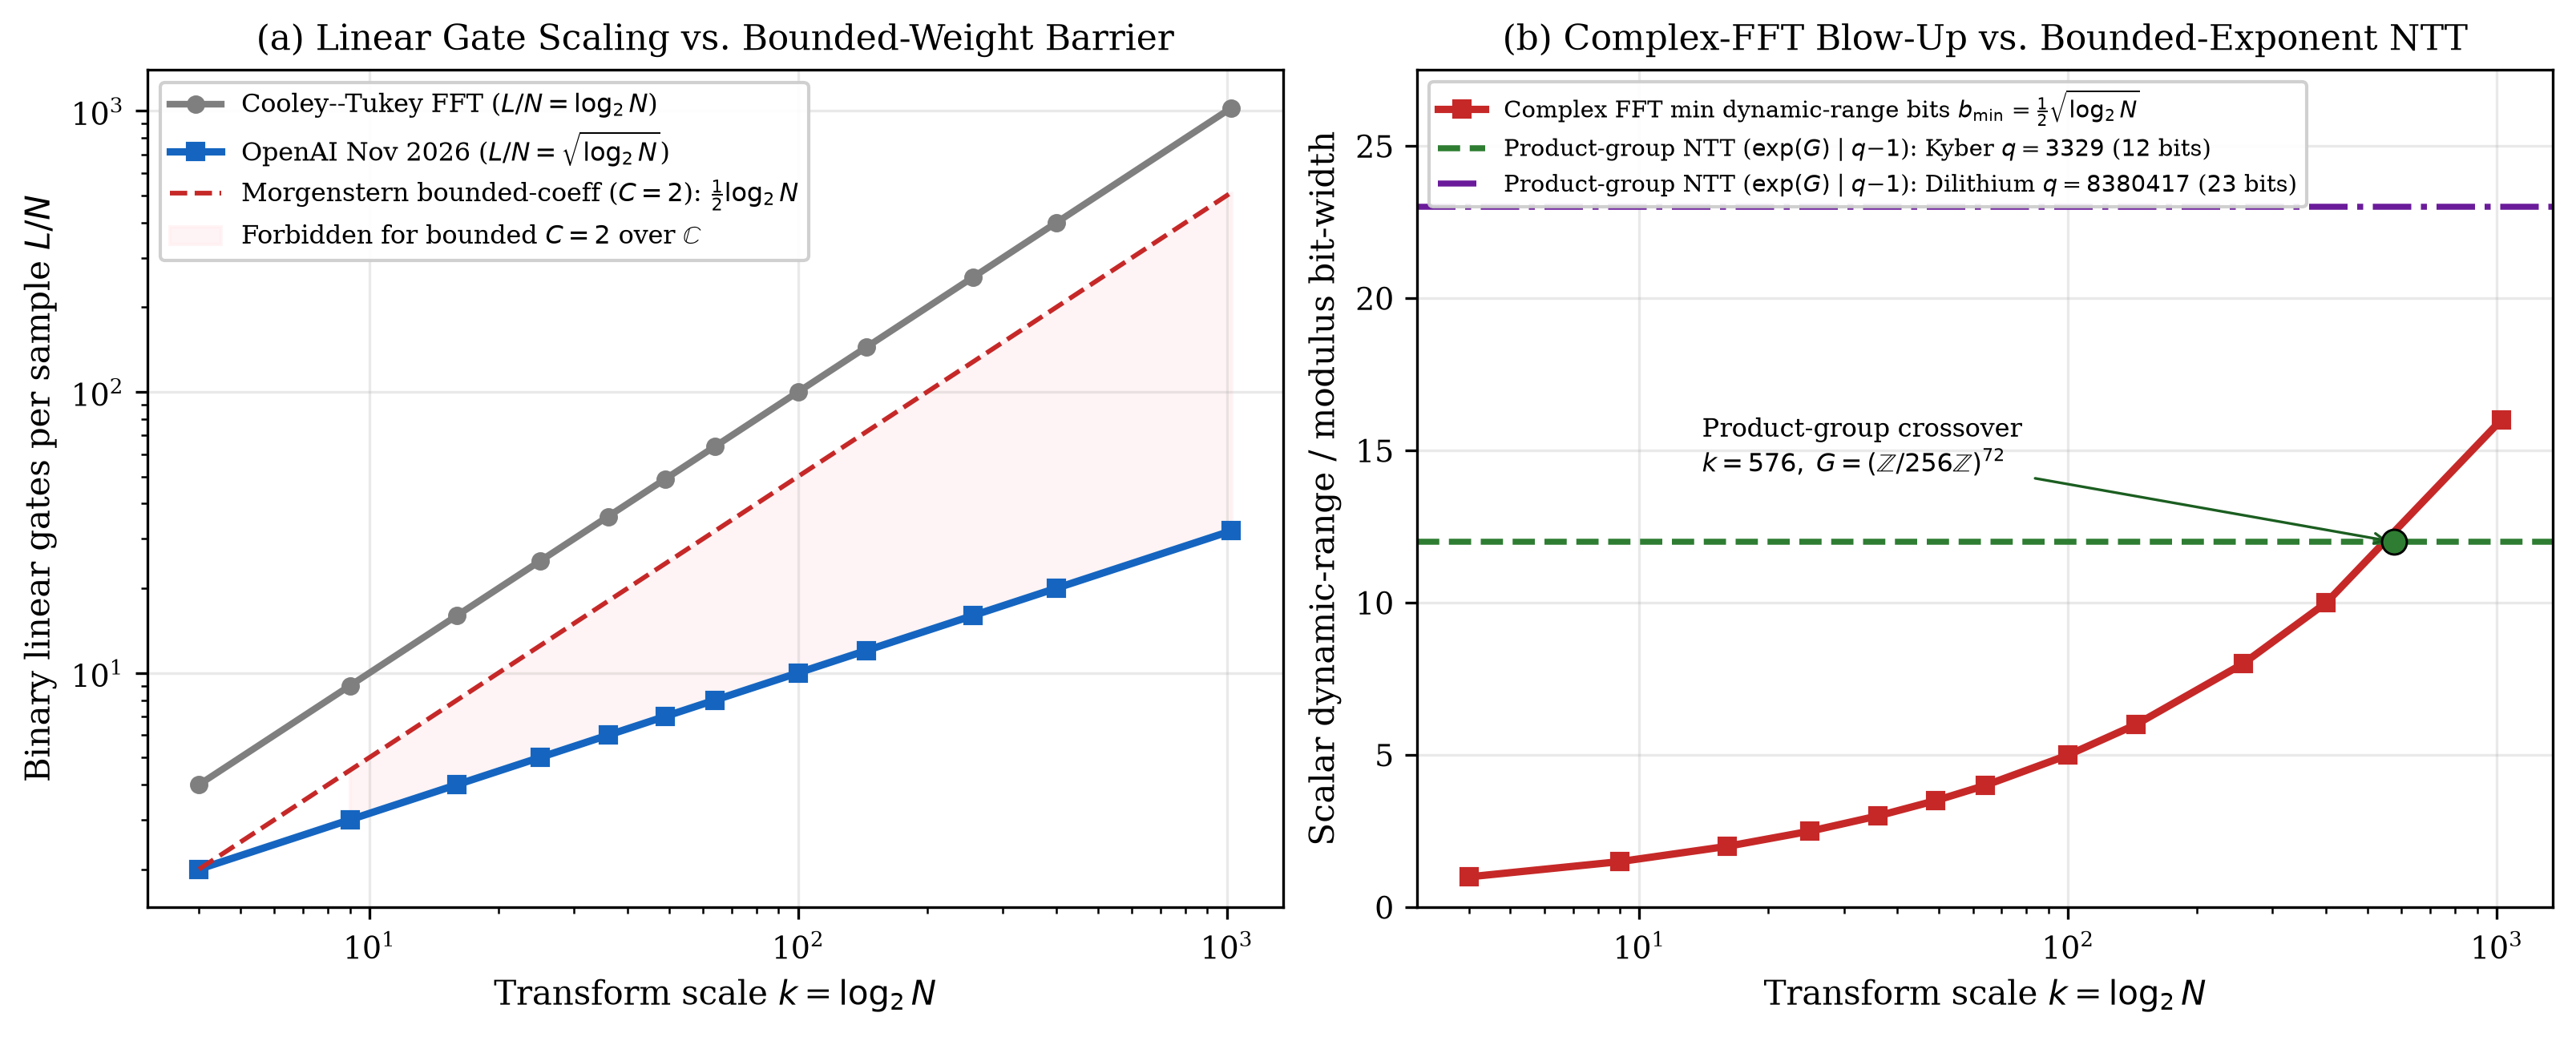
\includegraphics[width=0.98\linewidth]{figures/fig1_morgenstern_conservation.png}
\caption{Morgenstern Gate--Bit Conservation Law. (a)~Sub-logarithmic $N\sqrt{\log_2 N}$ gate counts enter the bounded-coefficient ($C=2$) forbidden zone over $\CC$. (b)~Minimum complex scalar dynamic-range bit-width $b_{\min} = \frac{1}{2}\sqrt{\log_2 N}$ grows unboundedly, crossing fixed-modulus bounded-exponent product-group NTTs ($\exp(G)\mid q-1$) over ML-KEM/Kyber $\FF_{3329}$ ($12$~bits) at $k = 576$ ($G = (\ZZ/256\ZZ)^{72}$).}
\label{fig:morg}
\end{figure}

\begin{figure}[t]
\centering
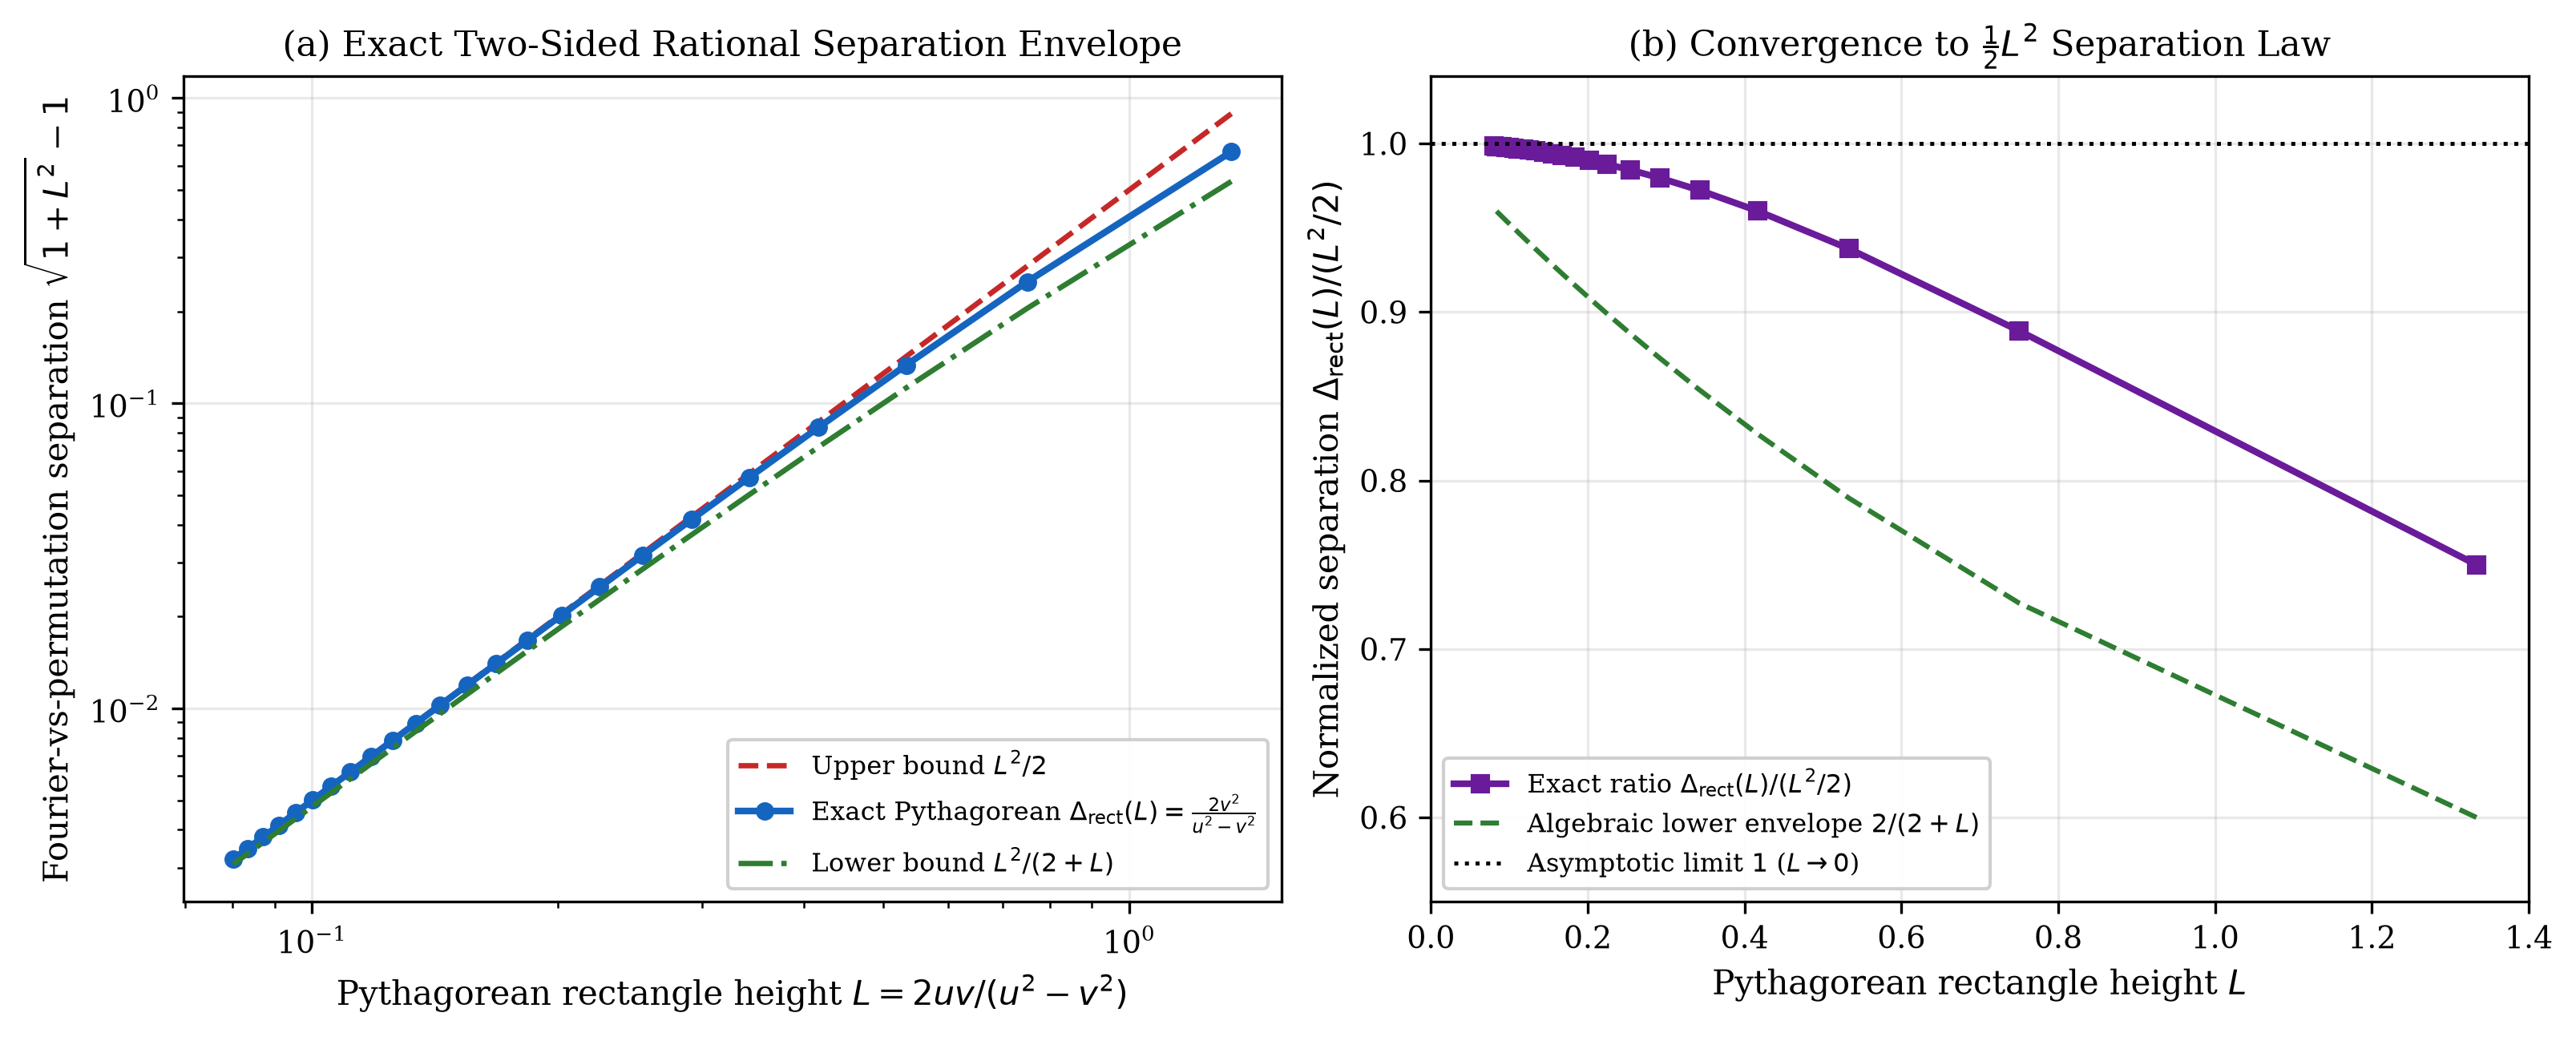
\includegraphics[width=0.98\linewidth]{figures/fig2_pythagorean_separation.png}
\caption{Exact Pythagorean rectangular rank--support separation. (a)~Exact rational values $\Delta_{\mathrm{rect}}(L) = 2v^2/(u^2-v^2)$ tightly bracketed between $L^2/(2+L)$ and $L^2/2$. (b)~Normalized ratio $\Delta_{\mathrm{rect}}(L)/(L^2/2)$ converging smoothly to $1$ as $L \to 0$.}
\label{fig:pyth}
\end{figure}

\begin{figure}[t]
\centering
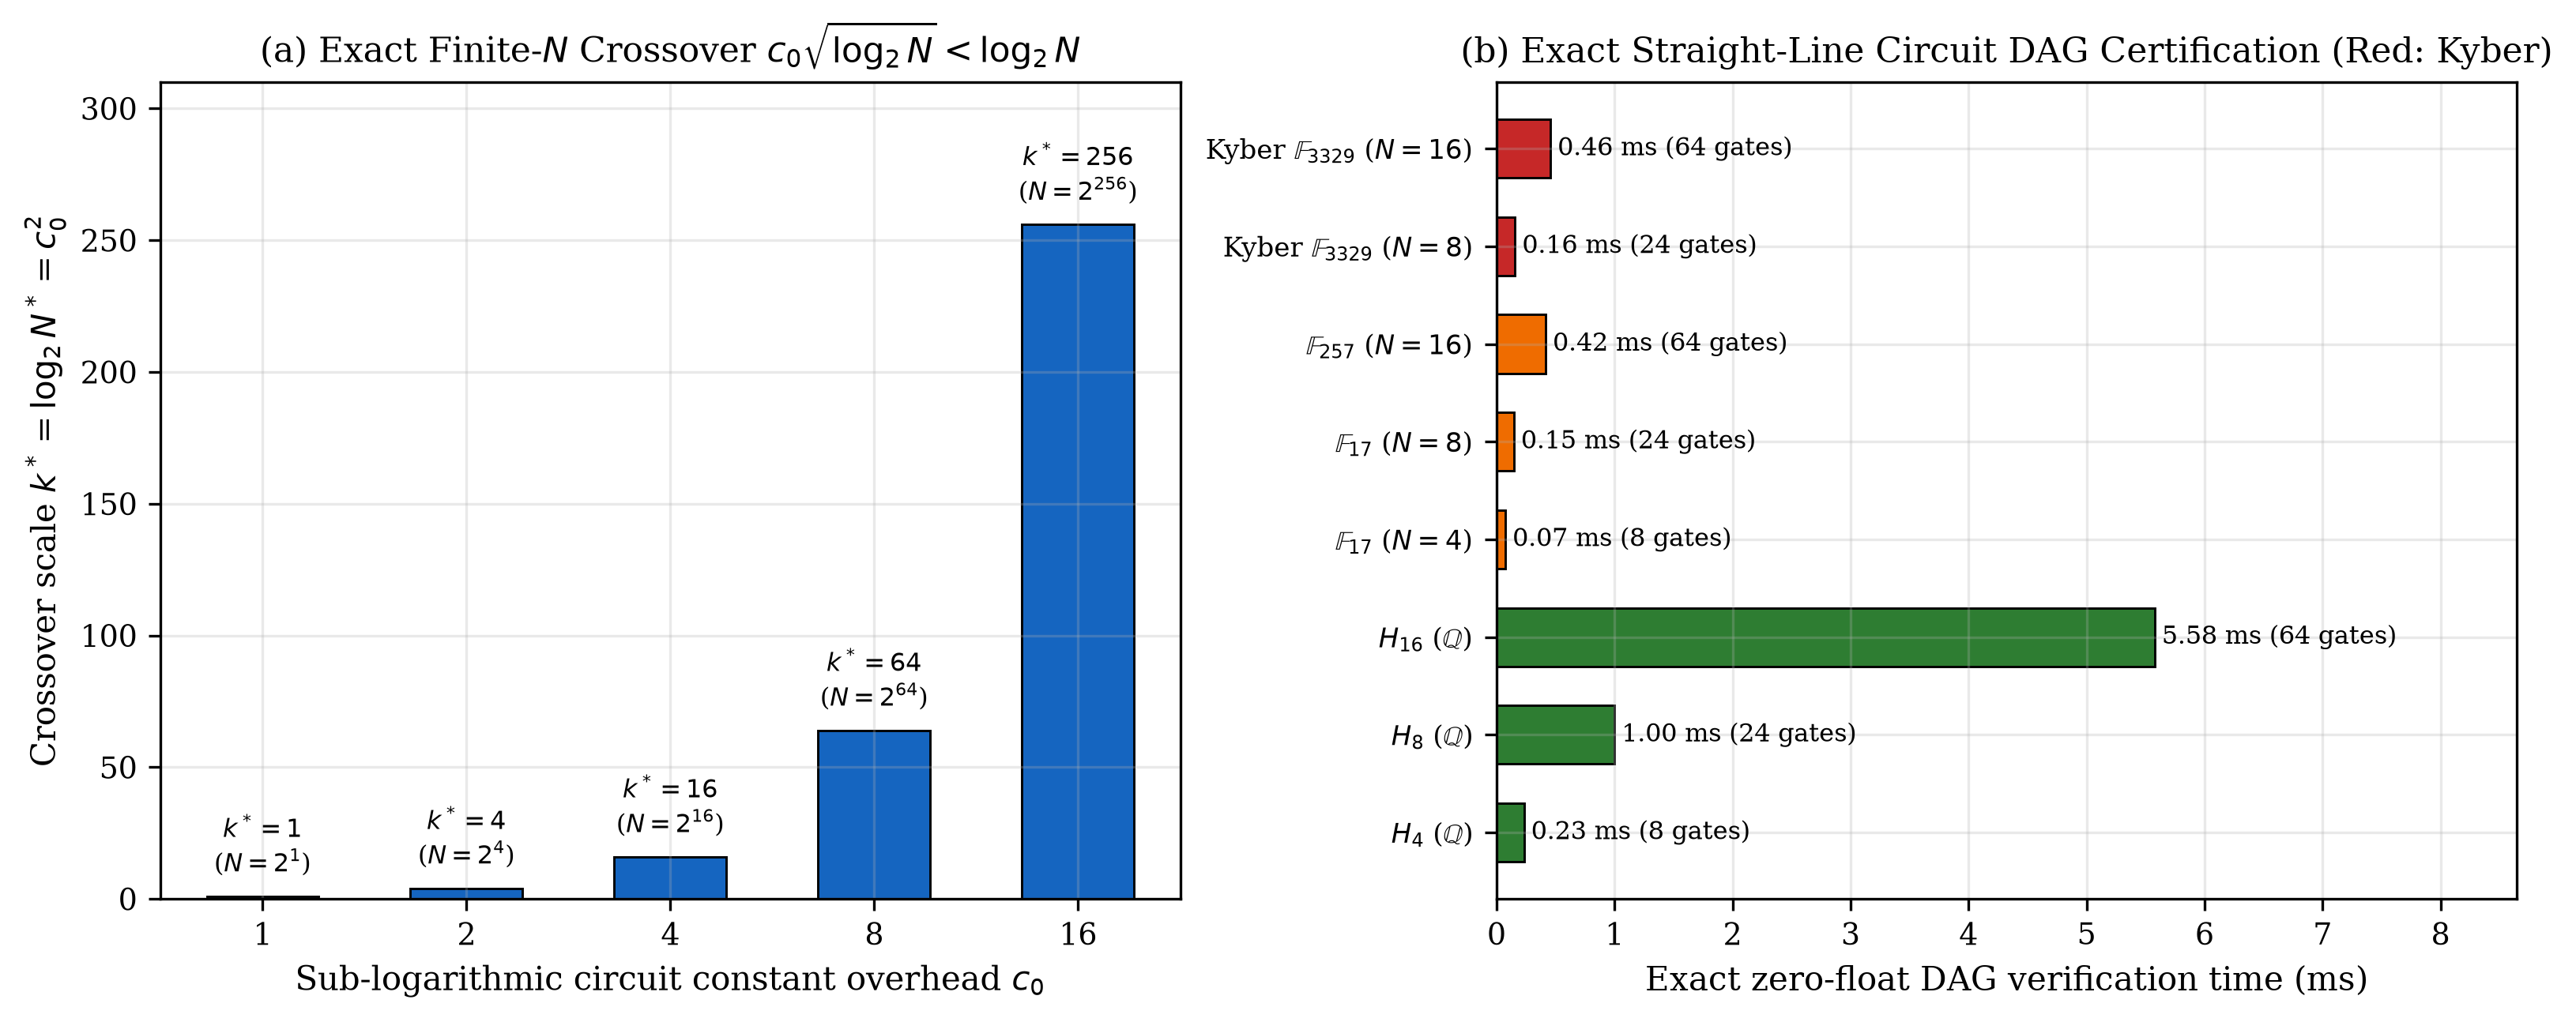
\includegraphics[width=0.98\linewidth]{figures/fig3_crossover_and_ntt_certs.png}
\caption{Finite-$N$ crossovers and exact DAG verification. (a)~Quadratic crossover scale $k^* = c_0^2$ where $c_0\sqrt{k} < k$. (b)~Zero-float verification times for exact acyclic classical Hadamard ($\QQ$) and post-quantum Kyber/Fermat NTT ($\FF_q$) circuit DAGs up to $N=16$.}
\label{fig:cross}
\end{figure}

\section{Limitations and Outlook}\label{sec:outlook}

Our Mode~3 and Mode~4 straight-line DAG certificates currently verify canonical $N\log_2 N$ Cooley--Tukey/Hadamard and NTT circuits up to $N \le 16$ via full $N$-basis simulation in $\le 5.58\,\mathrm{ms}$ ($H_{16}$ in $5.578\,\mathrm{ms}$, Kyber $\FF_{3329}$ $N=16$ in $0.457\,\mathrm{ms}$); they do not yet instantiate an explicit sub-logarithmic $N(\log_2 N)^{1/2+o(1)}$ prime-tensor-power circuit from~\cite{openai2026dft}, whose crossover occurs only at large $N$ ($k > c_0^2$). Extending exact verification to explicit sub-logarithmic circuits at larger $N$ will require randomized Freivalds or polynomial-identity checking combined with sparse DAG evaluation, and characterizing the concrete constant $c_0$ for bounded-exponent product-group NTTs over $\FF_{3329}$ and $\FF_{8380417}$ remains an open engineering challenge.

\bibliographystyle{plain}
\bibliography{references}

\end{document}
